% Chapter 4

\chapter{\uppercase{IMPLEMENTATION}} % Main chapter title
\label{chap4} % For referencing

\begin{spacing}{1.5} 
\begin{sloppypar}

In this chapter, we will discuss the implementation details of Autonomous Driving agent.
\section{ENVIRONMENT}

In fig. \ref{fig:4way}, you can see the a different map. There are 10 such different maps in the Duckietown simulator. We can built custom maps too. In fig. \ref{fig:loop_dyn_duckiebots}, you can see cart. This cart is a dynamic object (It moves as time passes).

DuckieTown Simulator is an innovative educational platform that merges the concepts of autonomous vehicles and gamified learning. Originating from the DuckieTown project, a university-led initiative for teaching robotics and artificial intelligence, the simulator provides a virtual environment where users can experiment with self-driving car algorithms. It is built on the Gym-Duckietown environment, which is a high-fidelity simulator written in Python and OpenGL, offering a customizable and interactive platform for users to test and develop their autonomous driving solutions.

The simulator is designed to reflect the complexities of real-world driving within a controlled setting, allowing for the testing of navigation, object detection, and control systems without the risks associated with physical vehicles. This is particularly useful for educational purposes, where students can learn about the intricacies of robotics software and hardware interaction in a safe and repeatable environment. The DuckieTown Simulator also serves as a research tool, providing a detailed and scalable environment to test advanced algorithms and behaviors before deploying them in real-world scenarios.

One of the key features of the DuckieTown Simulator is its integration with the Robot Operating System (ROS), which is a flexible framework for writing robot software. This integration allows for a seamless transition from simulation to real-world application, as the same code base can be used in both virtual and physical Duckiebots. The simulator supports various experiments, including reinforcement learning, where agents can be trained to navigate through the DuckieTown with the goal of reaching a destination efficiently while obeying traffic rules and avoiding obstacles.

Moreover, the DuckieTown Simulator is not just a tool for individual learning but also facilitates collaborative projects and competitions. It enables users from around the globe to participate in challenges that test the limits of their coding and problem-solving skills in a fun and engaging way. The simulator's open-source nature encourages community contributions, leading to continuous improvements and updates that enhance its capabilities and educational value.

In conclusion, the DuckieTown Simulator represents a significant advancement in the field of robotics education and research. It provides a bridge between theoretical knowledge and practical application, fostering a deeper understanding of autonomous systems. By offering a realistic and accessible platform, it empowers enthusiasts, students, and researchers alike to explore the future of mobility and autonomy. The simulator's contribution to the democratization of robotics education cannot be overstated, as it lowers the barriers to entry and allows a wider audience to engage with cutting-edge technology.
\begin{figure}
    \centering
    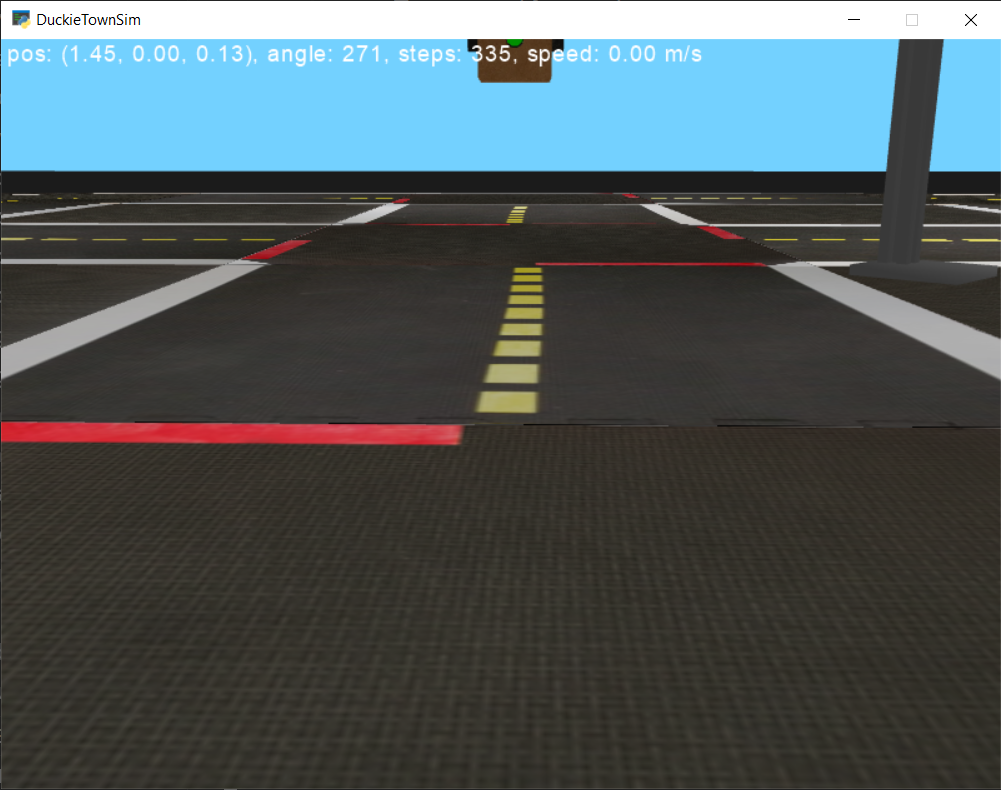
\includegraphics[width=1\linewidth]{4/4way.png}
    \caption{4way Environment}
    \label{fig:4way}
\end{figure}

% \subsection{loop\_dyn\_duckiebots}
\begin{figure}
    \centering 
    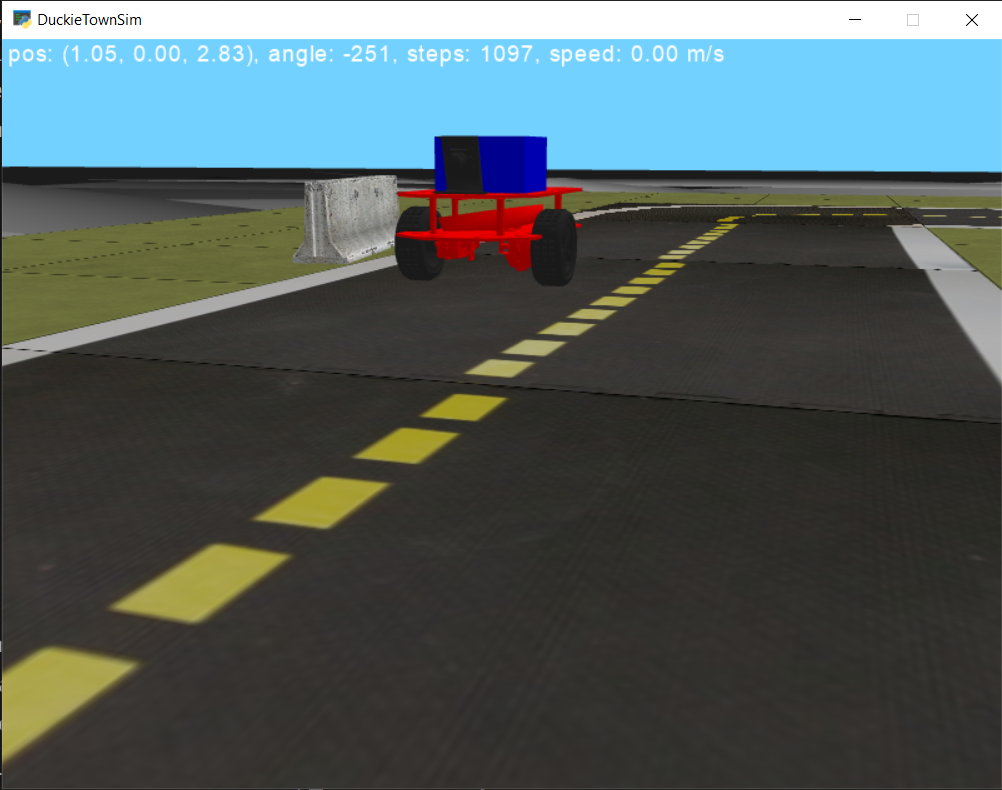
\includegraphics[width=1\linewidth]{4/loop dyn bots.png}
    \caption{Loop\_dyn\_duckiebots Environment}
    \label{fig:loop_dyn_duckiebots}
\end{figure}

\section{DATASET}

In fig \ref{fig:processed_dataset}, we can see the dataset generate by the Dataset Collection Tool. It is stored in .pkl format. The dataset's columns are: i) Video Description, ii) Action to take, iii) Reasoning and iv) predict the next control signals.

Dataset Preparation:
\begin{itemize}
    \item Collect a diverse set of videos relevant to the task at hand.
    \item Annotate the videos with frame-level labels if necessary for supervised learning.
    \item Preprocess the videos to a consistent format and resolution.
    \item Split the dataset into training, validation, and test sets.
\end{itemize}


\begin{figure}
    \centering 
    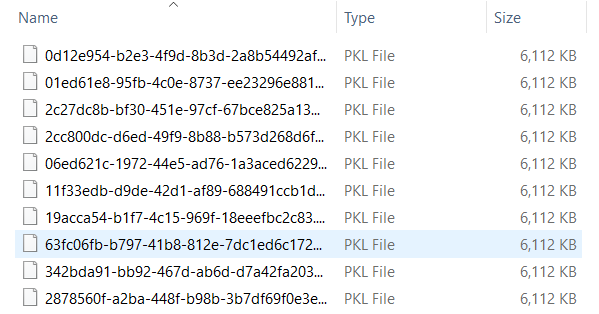
\includegraphics[width=1\linewidth]{4/processed_dataset.png}
    \caption{Dataset}
    \label{fig:processed_dataset}
\end{figure}
\section{VISION ENCODER}
In \ref{algo:encoder}, we can see the algorithm for Vision Encoder. The vision encoder is implemented in pure python using pytorch's submodules such as nn.Module, autograd etc.

The alignment head is implemented using nn.Module and is train on the above collected dataset. The tokenizer and Embedding model is provided by the LLM Module. We are using Swin Transformer for video feature extraction.
\begin{algorithm}
\caption{Video Encoder Architecture}
\begin{algorithmic}
\State \textbf{Input:} Images
\State \textbf{Output:} Video Representation
\State \textbf{Algorithm:}
\State \indent \textbf{Preprocess}
\State \indent \indent Concat the $N$ context sequence images
\State \indent \indent Split the images into smaller $pm1 \times pm2$ image patches
\State \indent \textbf{Linear Projection}
\State \indent \indent Apply Positional Embedding
\State \indent \indent Apply Patch Embedding
\State \indent \indent Concat Positional Embeddings and Patch Embeddings for each Patch
\State \indent \textbf{Vision Transformer} $\to Video Representation$ 

\end{algorithmic}
\label{algo:encoder}
\end{algorithm}

\section{DATA COLLECTION TOOL}
The Data Collection Tool has 2 sub-modules. Their implementations are discussed below

\subsection{Recorder}
In \ref{algo:recorder}, you can see the algorithm of Recorder sub-module in Data Collection Module.
\begin{algorithm}
\caption{Data Recorder Algorithm}
\begin{algorithmic}
\State \textbf{Input:} Screen
\State \textbf{Output:} Clip list
\State \textbf{Algorithm}
\State \indent Focus the window with the title 'Duckietown Sim'
\State \indent Get the window corner coordinates
\State \indent Create a clip list
\State \indent Repeat number of frames per clip times
\State \indent \indent Get screenshot of the window 
\State \indent \indent Add it to the screenshot to the clip list
\State \indent \indent Wait 1//fps secs
\State \indent Return Clip list

\end{algorithmic}
\label{algo:recorder}
\end{algorithm}
\subsection{Data Annotation Tool}  
the data annotation tool is implemented using pysimplegui. A proprietary GUI library in python that is free for use for non-commercial academic purposes. The tool will be replaced by a flask web app for ease of use, accessibility and open-source natures.
\section{CONTROL MODULE}
The Control module is a simple python script which which looks for words such as 'accelerate', 'decelerate', 'turn left' and 'turn right'. Then, converts that words into key presses corresponding to the word given. This is parsed from the model's output parameter 'predicted next control signal'. The current dataset is of the list format which makes it difficult to parse. In future, the format is to be changed to json format.

\end{sloppypar}
 \end{spacing}

